\documentclass{beamer}

% Top-aligning columns within a top-aligned frame
% https://tex.stackexchange.com/questions/16447/beamer-top-aligning-columns-within-a-top-aligned-frame
\makeatletter
\newenvironment{myitemize}{%
   \setlength{\topsep}{0pt}
   \setlength{\partopsep}{0pt}
   \renewcommand*{\@listi}{\leftmargin\leftmargini \parsep\z@ \topsep\z@ \itemsep\z@}
   \let\@listI\@listi
   \itemize
}{\enditemize}
\makeatother  

\usepackage[USenglish]{babel}
\usepackage[utf8]{inputenc}
\usepackage{amssymb, amsmath}
\usepackage{bm}
\usepackage{color}
\usepackage{tikz}
\usepackage{url}

\definecolor{links}{HTML}{2A1B81}
\hypersetup{colorlinks,linkcolor=,urlcolor=links}

\usetheme{Boadilla}

\bibliographystyle{apalike}
% make bibliography entries smaller
%\renewcommand\bibfont{\scriptsize}
% Now get rid of all the colours
\setbeamercolor*{bibliography entry title}{fg=black}
\setbeamercolor*{bibliography entry author}{fg=black}
\setbeamercolor*{bibliography entry location}{fg=black}
\setbeamercolor*{bibliography entry note}{fg=black}

\newcommand{\lnorm}[1]{\left\lVert#1\right\rVert^2}
\newcommand{\norm}[1]{\left\lVert#1\right\rVert}

% and kill the abominable icon
\setbeamertemplate{bibliography item}{}

\begin{document}
\title[BigBird]{RandAugment: Practical automated data augmentation with a reduced search space}  
\author{Radek Bartyzal}
\date{22. 9. 2020} 
\institute{GLAMI AI}

\frame{\titlepage} 

%--------- END Frame 12 -------------
\begin{frame}{Motivation}

Training data augmentation = good.
\vfill
How to make it better?

\begin{itemize}
\item tailor the augmentations to your net + dataset
\item $\implies$ training the augmentation transformation 
\end{itemize}

\end{frame}
%--------- END Frame 12 -------------
\begin{frame}{Previous works}

\textbf{AutoAugment} \cite{cit:auto}
\begin{itemize}
\item 14 image transformation functions: f(image, magnitude)
\item configure 30 parameters:
\begin{itemize}
\item prob of choosing each transformation = 14 params
\item magnitude of each transformation = 14 params
\end{itemize}
\item params were chosen by running hyper param search on a proxy task
\item proxy task = smaller net + subset of train dataset
\end{itemize}
\end{frame}
%--------- END Frame 12 -------------
\begin{frame}{RandAugment}

\begin{itemize}
\item 14 image transformation functions: f(image, magnitude)
\item selects all image transformations with
equal probability
\item only 2 params:
\begin{itemize}
\item[N:] number of randomly selected transformations
\item[M:] magnitude of all transformations
\end{itemize}
\item $\implies$ can be used as hyper-params during full training
\item $\implies$ no proxy task, directly optimize for the final net
\end{itemize}

\end{frame}
%--------- END Frame 12 -------------
\begin{frame}{RandAugment code}

\begin{figure}[h]
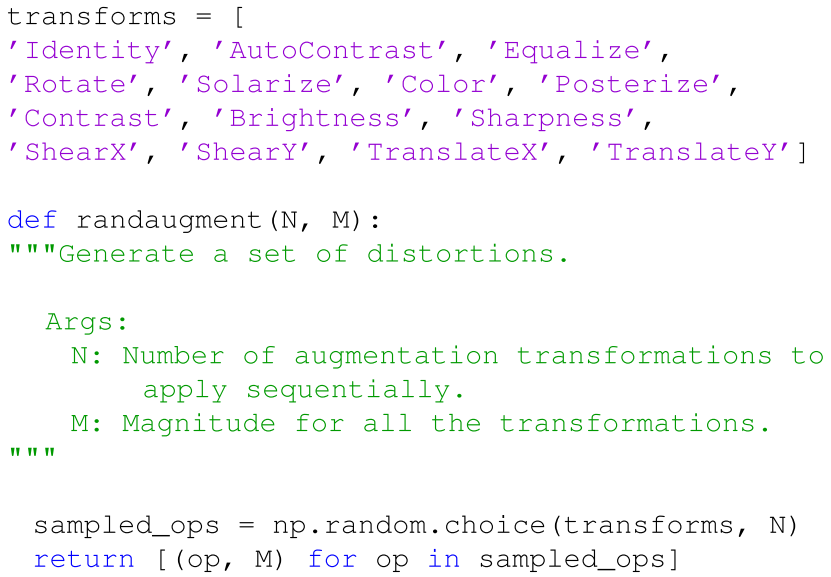
\includegraphics[width=0.8\textwidth]{img/code}
\caption{Only 2 params: $N$ and $M$.}
\end{figure}

\end{frame}
%--------- END Frame 12 -------------
\begin{frame}{Results: ImageNet}
\begin{figure}[h]
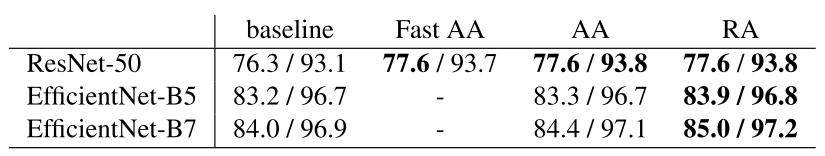
\includegraphics[width=\textwidth]{img/imagenet}
\caption{Top-1 and Top-5 accuracies (\%) on ImageNet. Baseline,  AutoAugment (AA), Fast AutoAugment (Fast AA) taken from sources (see paper).}
\end{figure}
\end{frame}
%--------- END Frame 12 -------------
\begin{frame}{Results: COCO}
\begin{figure}[h]
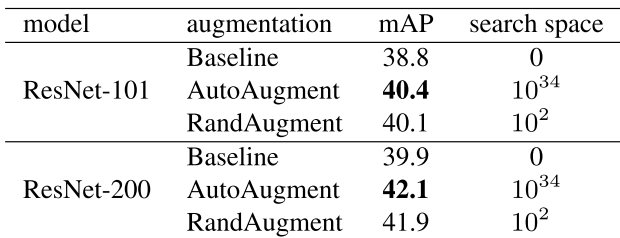
\includegraphics[width=0.8\textwidth]{img/coco}
\caption{Mean average precision (mAP) on COCO detection task. Search space size is reported as the order of magnitude of the number of possible augmentation policies. Models are trained for 300 epochs from random initialization.}
\end{figure}
\end{frame}
%--------- END Frame 12 -------------
\begin{frame}{Adding possible transformations improves accuracy}
\begin{figure}[h]
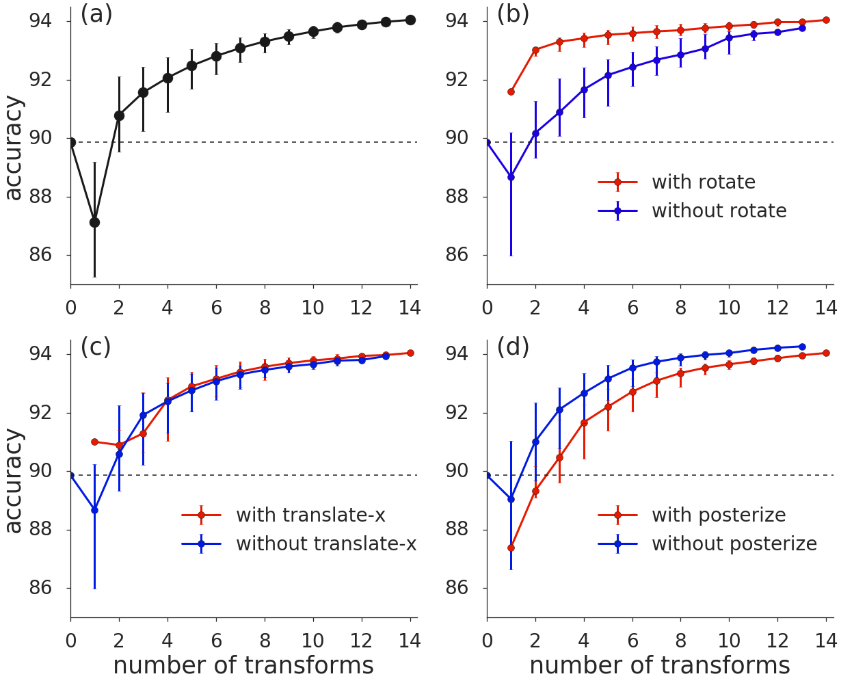
\includegraphics[width=0.6\textwidth]{img/N}
\caption{Median CIFAR-10 validation accuracy for Wide-ResNet-28-2 model architectures trained with RandAugment (N = 3, M = 4) using randomly sampled subsets of transformations. No other data augmentation is included in training. Dashed line = no augmentations. Posterize hurts accuracy.}
\end{figure}
\end{frame}
%--------- END Frame 12 -------------
\begin{frame}{Conclusion}

\end{frame}

%--------- END Frame 12 -------------
\begin{frame}{Sources}
\begin{thebibliography}{0}

  \bibitem[1]{cit:paper} 1. Cubuk, Ekin D., et al. "Randaugment: Practical automated data augmentation with a reduced search space." Proceedings of the IEEE/CVF Conference on Computer Vision and Pattern Recognition Workshops. 2020. \url{https://arxiv.org/abs/1909.13719} 
  
   \bibitem[2]{cit:auto} 2. Cubuk, Ekin D., et al. "Autoaugment: Learning augmentation policies from data." arXiv preprint arXiv:1805.09501 (2018). \url{https://arxiv.org/abs/1805.09501} 
   
\end{thebibliography}
\end{frame} 
\end{document}
